% APÊNDICES--------------------------------------------------------------------

\begin{apendicesenv}
\partapendices



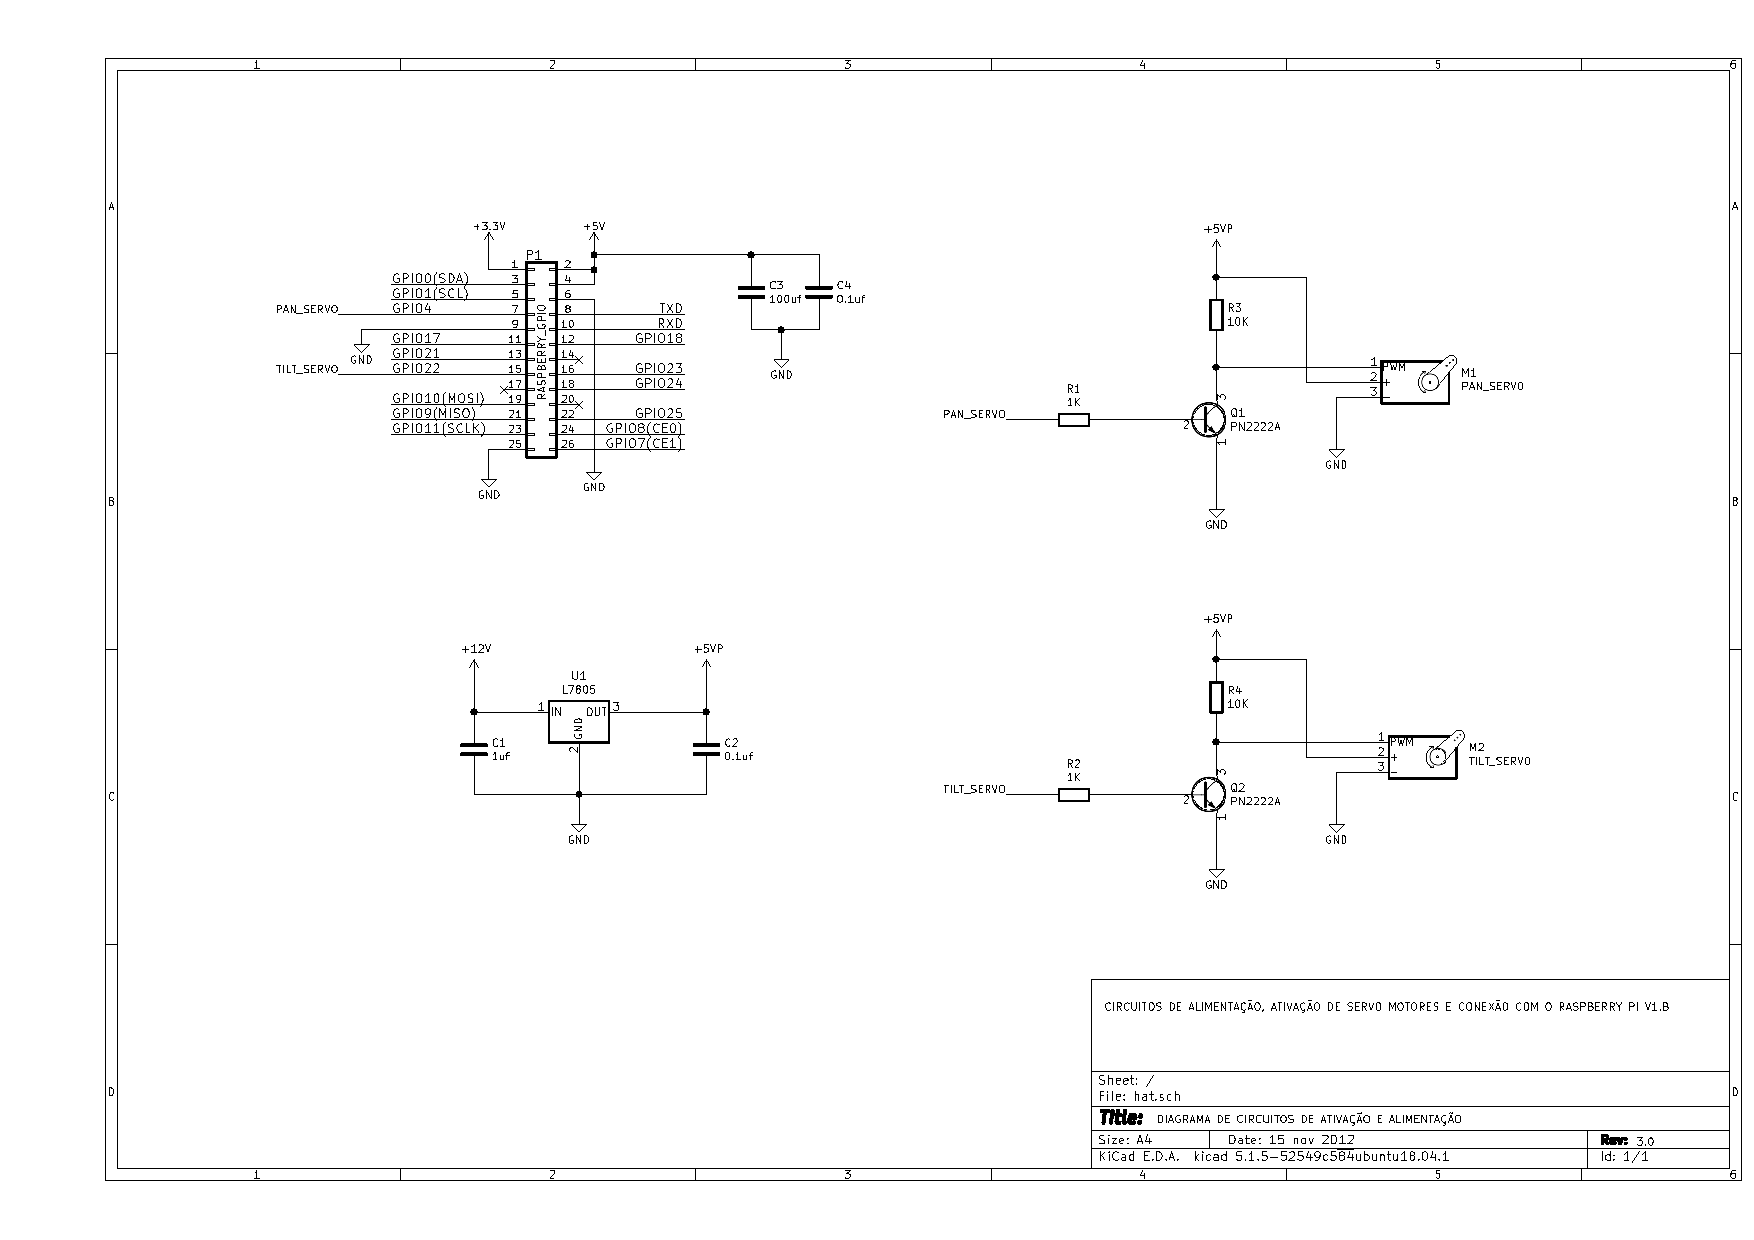
\includepdf[pages=-,offset=0 -20,angle=-90,scale=0.9,pagecommand={
	\chapter{Diagrama de Circuitos} % Edite para alterar o título deste apêndice
	\label{chap:board}
}]{../board/hat.pdf}

\chapter{Fotos do Protótipo} % Edite para alterar o título deste apêndice
\label{chap:fotosprototipo}

\begin{figure}[H]
	\centering
	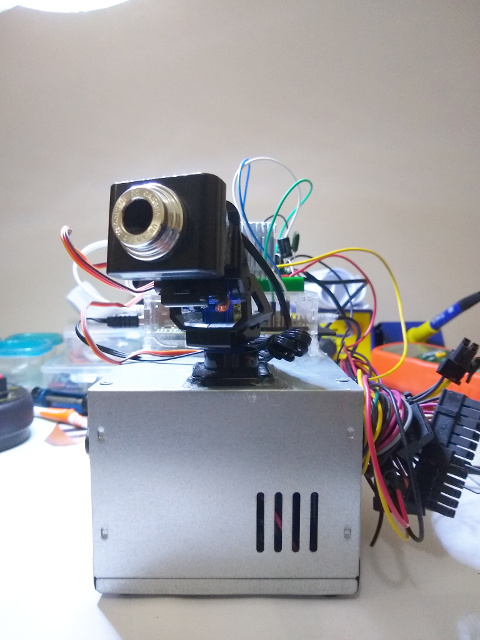
\includegraphics[width=1\linewidth]{figuras/vista_frontal}
	\caption{Visão frontal.}
	\label{fig:vistafrontal}
\end{figure}

\begin{figure}[H]
	\centering
	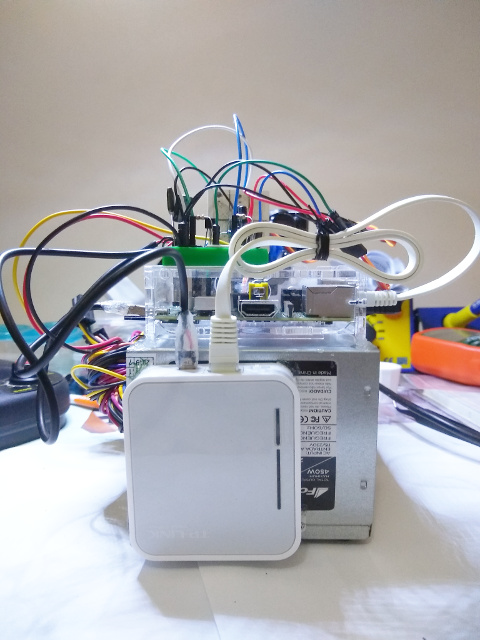
\includegraphics[width=1\linewidth]{figuras/vista_traseira}
	\caption{Visão traseira.}
	\label{fig:vistatraseira}
\end{figure}

\begin{figure}[H]
	\centering
	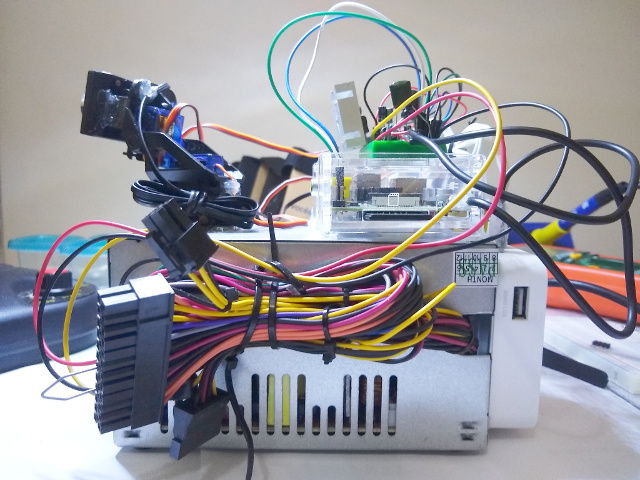
\includegraphics[width=1\linewidth]{figuras/vista_esquerda}
	\caption{Visão lateral esquerda.}
	\label{fig:vistaesquerda}
\end{figure}

\begin{figure}[H]
	\centering
	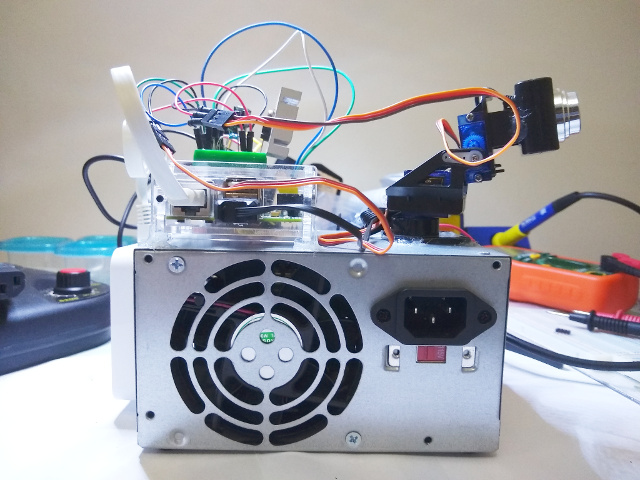
\includegraphics[width=1\linewidth]{figuras/vista_direita}
	\caption{Visão lateral direita.}
	\label{fig:vistadireita}
\end{figure}

\begin{figure}[H]
	\centering
	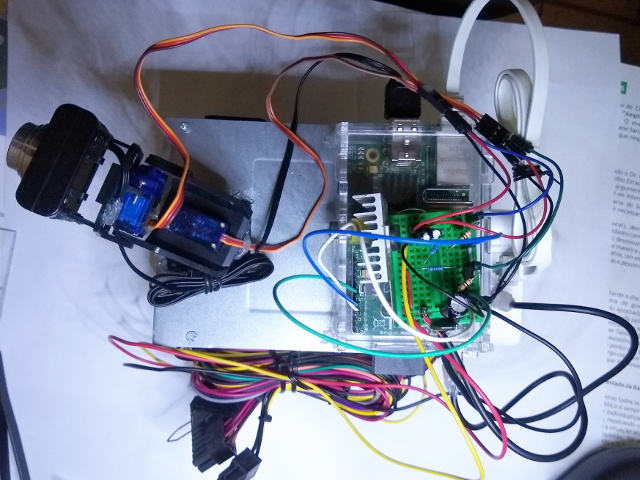
\includegraphics[width=1\linewidth]{figuras/vista_superior}
	\caption{Visão superior.}
	\label{fig:vistasuperior}
\end{figure}

\begin{figure}[H]
	\centering
	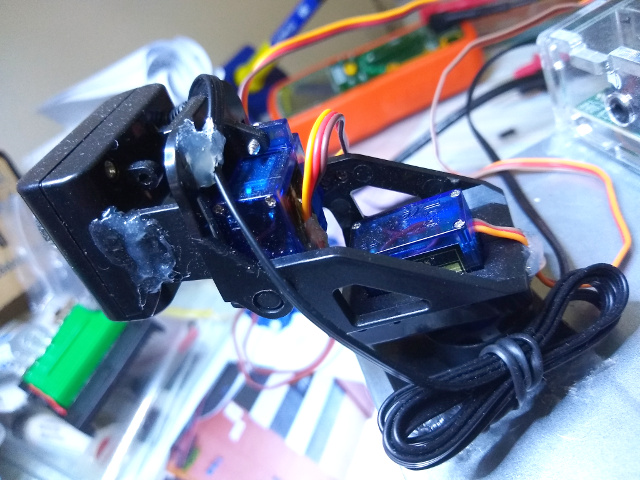
\includegraphics[width=1\linewidth]{figuras/vista_detalhe_fixacao_camera}
	\caption{Fixação da câmera com cola quente.}
	\label{fig:vistadetalhefixacaocamera}
\end{figure}

\begin{figure}[H]
	\centering
	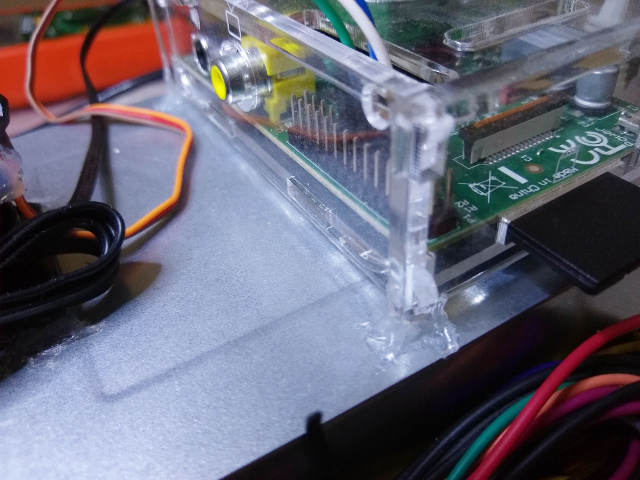
\includegraphics[width=1\linewidth]{figuras/vista_detalhe_fixacao_raspi}
	\caption{Fixação do gabinete do \textit{Raspberry Pi} com cola quente.}
	\label{fig:vistadetalhefixacaoraspi}
\end{figure}

\begin{figure}[H]
	\centering
	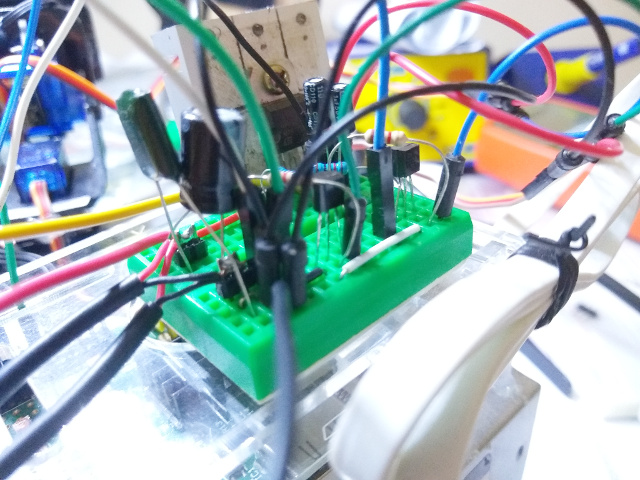
\includegraphics[width=1\linewidth]{figuras/vista_detalhe_circuito}
	\caption{Detalhe da montagem do circuito na mini \textit{breadboard}.}
	\label{fig:vistadetalhecircuito}
\end{figure}

\end{apendicesenv}
